

\newcommand{\absentPerc}{80.0} %
\newcommand{\absentEngPerc}{61.3} %
\newcommand{\absentEngOneKPerc}{48.8} %
\newcommand{\gapsPerc}{81.8} %
\newcommand{\pregapsPerc}{76.5} %
\newcommand{\midgapsPerc}{7.4} %
\newcommand{\postgapsPerc}{16.1} %

\newcommand{\midgapsPossPerc}{29.8} %
\newcommand{\midgapsDomainsPerc}{54.1} %
\newcommand{\lifespanNoGaps}{11.2} %
\newcommand{\lifespanGaps}{16.5}

\newcommand{\numpresentdoms}{108,499} %
\newcommand{\numabsentenglishdoms}{150,192}



\newcommand{\midgapNoRankPerc}{3.0}
\newcommand{\pregapNoRankPerc}{78.4}
\newcommand{\postgapNoRankPerc}{11.2}
\newcommand{\allgapNoRankPerc}{92.7}
\newcommand{\notgapNoRankPerc}{7.3}

\newcommand{\percSnapshotWithPrior}{85.3} %
\newcommand{\percSnapshotWithoutPrior}{14.7} %


\newcommand{\corrMidgap}{-0.02} %
\newcommand{\corrPregap}{0.07} %
\newcommand{\corrPostgap}{0.08} %

\newcommand{\nSnapshots}{910,546}
\newcommand{\nSites}{108,499}


\section{Corpus composition}
\label{sec:ppot:dataset}

In order to understand the structure and biases of the data, we discuss the dataset composition.

\subsection{Cleaning the corpus}
\label{sec:ppot:deduplication}
In order to ensure the quality of our analysis, we purged additional, real policies from our dataset that might lead to a biased analysis. In total, we removed 160,941 policies following the steps listed below, leaving us with 910,546 policies from 108,499 sites. We call the resulting corpus the \textit{analysis subcorpus}. In sections \ref{sec:ppot:dataset}, \ref{sec:ppot:doclevstatstime}, and \ref{sec:ppot:analysis} we use the analysis subcorpus for our analyses.\footnote{While we removed this data for our analyses, we anticipate that there may be some research questions that would benefit from their inclusion. Accordingly, in our public release, we include both the full corpus and the analysis subcorpus.} 

\textbf{Parked domains.} As our dataset spans more than 20 years,
many domains have expired and were parked for monetization.
We found that privacy policies of the parking services such as {\tt godaddy.com} and {\tt hugedomains.com} were abundant in our dataset as they hosted privacy policies of 7,092 and 2,275 distinct domains, respectively.
We built a detection method based on the lists of domain parking services and registrars from prior research~\cite{vissers2015parking, kuhrer2014paint, kuhrer2014paint-TR, wang2006strider},
and the ICANN-Accredited Registrars list~\cite{ICANN-Registrars}.
With this method, we detected 79 parking providers and resellers and removed 24,289 (2.3\%) snapshots hosted by these providers.
 
\textbf{Homepage redirection.} In order to ensure the metadata is consistent with policy content, we removed policy snapshots with a cross-origin homepage redirection (COHR), unless both sites were likely owned by the same entity. Thus, we removed COHR policy snapshots, but we made an exception for websites with
common~\emph{label}s in their domain names (e.g. \texttt{google.com} and \texttt{google.ca})
as this may indicate that they are owned by the same organization.

\textbf{Policy URL.} Finally, to remove duplicates, we followed
Degeling et al.'s approach based on privacy policy URLs~\cite{degeling2018we}. When two or more sites shared a policy URL during the same interval, we kept only one, preferring the snapshot where the homepage domain matched the privacy policy domain. This removed 61,220 policies.





\subsection{Corpus overview}
\label{subsec:ppot:data-overview}

\begin{figure}[]
\centering
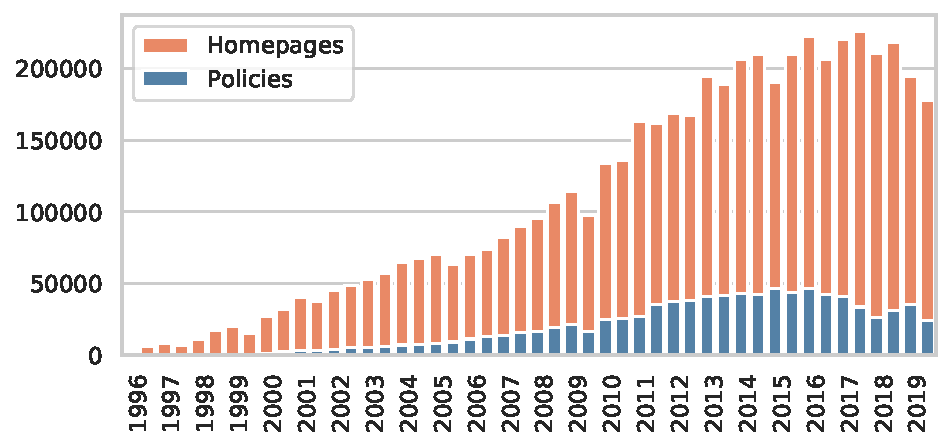
\includegraphics[width=0.99\columnwidth]{chapters/privacypolicies/figures/policy_homepage_counts.pdf}
\caption{The number of homepage snapshots and privacy policies for each interval. Note that each bar represents one interval and there are two intervals per year.}
%\Description[Bar plot of homepages versus policies, by year]{Generally, there are many more homepages than policies. The number of policies peaks in 2015 but declines slightly. The number of homepages roughly matches the same trend as the number of policies. }
\label{fig:numpolicies}
\end{figure}

On average, a website has 8.4 privacy policy snapshots ($M=6$). Although the dataset contains policies from as early as 1997, 79.4\% of the policies are from snapshots archived in 2010 or later.
As we briefly explored in Section~\ref{subsec:ppot:failure-analysis}, we expected the rate of successful downloads from earlier snapshots to be lower, in part due to different website structures, such as greater use of frames.

Figure~\ref{fig:numpolicies} shows the number of privacy policies and homepage snapshots per interval.
The decreases in the number of policies in 2009B and 2018A also occur in the number of homepage snapshots in those intervals, indicating that these decreases are due to changes in archiving or incomplete archives for those intervals.

\begin{figure}[t]
\centering
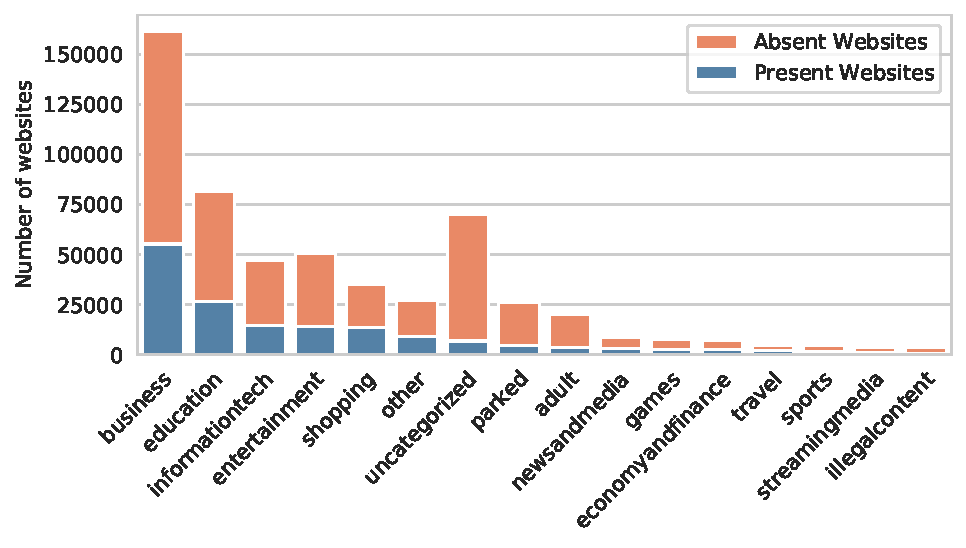
\includegraphics[width=1\columnwidth]{chapters/privacypolicies/figures/category_dist.pdf}

\caption{The distribution of website categories for present and missing sites. ``Other'' is composed of the 27 least frequent categories for English language websites. Websites which belong to multiple categories are counted once per category. Websites with no listed categories are added to the ``uncategorized'' category.}
%\Description[Histogram of category vs number of websites]{This diagram shows the number of websites that we tried to capture and that we succeeded in extracting an English language policy from. Categories in descending order: business, education, informationtech, entertainment, shopping, other, uncategorized, parked, adult, newsandmedia, games, economyandfinance, travel, sports, streamingmedia, illegalcontent.}
\label{fig:cat_dist}
\end{figure}

{\textbf{Distribution of website categories.}}
We examined the website categories for which we have the best coverage. We collected category data from Webshrinker~\cite{Webshrinker}, which provides a domain category lookup API.
Because category data is not available historically from Webshrinker, we assumed that categories are constant across time. We collected category data for the \numpresentdoms~websites in our dataset (present) and an additional \numabsentenglishdoms~websites with English homepages that were at one point in the Alexa top 100K (absent), which we show in Figure~\ref{fig:cat_dist}.
Just a few categories dominate both our dataset and English websites in general, and uncategorized websites are strongly underrepresented in our dataset.

{\textbf{Distribution of snapshot Alexa ranks.}}
The distribution of homepages and snapshots by Alexa rank is shown in Table~\ref{tab:rate-of-download-per-rank-bin}.
The >1M bin contains snapshots for which we do not have an Alexa rank, either because they were not listed in the Alexa top 1M or were captured
before 2009.
While the majority of our policies come from websites with rank 100K and up, the success rate of obtaining a policy is much higher if the website is in the top 10K. 

\begin{table}[]
\centering
\resizebox{0.9\columnwidth}{!} \\ \midrule
(1, 1K{]}       & 13,455   & 5,003   & 37.2 \\
(1K, 10K{]}     & 104,801  & 38,959  & 37.2 \\
(10K, 100K{]}   & 980,928  & 278,324 & 28.4 \\
(100K, 1M{]}    & 1,339,157 & 319,866 & 23.9 \\
\textgreater 1M & 2,786,853 & 268,394 & 9.6  \\ \bottomrule
\end{tabular}%
}
\caption{Rate of successful privacy downloads per Alexa rank buckets -- based on privacy policies in the analysis subcorpus.}
\label{tab:rate-of-download-per-rank-bin}
\end{table}

